\documentclass{article}
\usepackage[utf8]{inputenc}
\usepackage{xcolor}
\usepackage{graphicx}
\usepackage{hyperref}
\usepackage[margin=1.5cm]{geometry}
\hypersetup{colorlinks=true,linkcolor=blue,urlcolor=blue}

\title{Project 1 CS384 -   GUI Based Marksheet Generator}
\author{Dr. Mayank Agarwal}
\date{Assignment Given: 17th Oct 2021,\\ Deadline 1st December 2021,  
23:59\\Submission: GitHub }
\begin{document}
	\maketitle  
	\textbf{Things to be kept in mind} 
	\begin{enumerate}
%		\item Dont take any inputs from user . 
\item You need to make the project in a group of 2 students. If you wish you 
can do individually also. 
\item Number of questions needs to be auto-computed based on the last 
column of the ANSWER roll number. 	

\item Ensure try catch is used so as to avoid issues while running the code. 

\item You can take online help, but you need to understand the code flow 
process.

\item Both partners need to commit the project to their respective github. 
\item Program will be checked for plagiarism.   
\end{enumerate}

When the quiz is conducted on Google Form, Google does not provide an option 
for computing -ve marking. It gives 0 marks for wrong answer. It just gives a 
csv file as output for post 
processing. Your task is to make a standalone GUI/web based interface that will 
have such an option. \textbf{Web based is a preferred method in this project. }

\begin{figure}
	\centering
	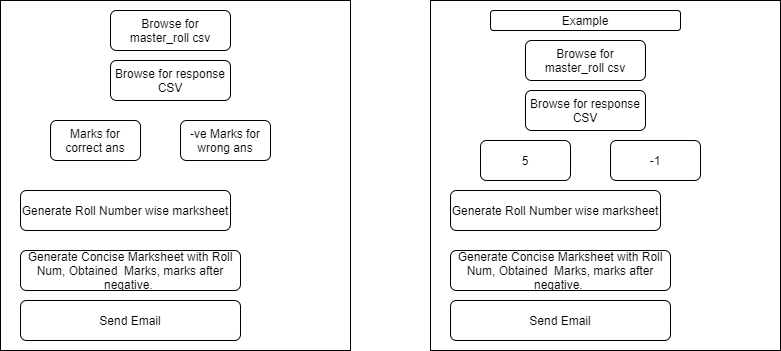
\includegraphics[width=0.99\linewidth]{Python_Project.png}
	\caption{GUI Options. On the right you are given the option for +ve and -ve 
	marks. In this example, it depicts that 5 mk are for correct answer, and -1 
	is for wrong. This input  should be dynamic, so calculations should be 
	based on the input provided. 0 is also a valid input for -ve case.}
	\label{fig:marksheet_project}
\end{figure}

\textbf{Input:}
You are given a \textbf{.csv} file that contains marks for each roll number and 
the individual options marked by each students(see sample 
input\textbackslash responses.csv). The 
following first seven 
columns are fixed: \\
\\
\textbf{Timestamp:}	At what time student submitted their question paper.\\
\textbf{Email address:}	Email address to which student login.\\       
\textbf{Score:}	Total calculated score.\\
\textbf{Name:}	Name of the student.\\
\textbf{IITP webmail:}	IITP webmail address.\\
\textbf{Phone number:} Phone number of the student\\
\textbf{Roll Number:} Roll number of the student.\\

\textbf{Outputs}
\begin{enumerate}
	\item Your aim is to make a GUI as shown in Figure 
	\ref{fig:marksheet_project}. Here 
	the first button is to upload a master\_roll.csv file. It contains the 
	names 
	and roll number of all the students of the class. (see sample 
	input\textbackslash  
	master\_roll.csv)
	
	\item Next is the response sheet csv obtained from google  (see sample 
	input\textbackslash  
responses.csv). You need to check that a row with roll number ANSWER should be 
present in this file. If not, pop and error saying that, ``no roll number with 
ANSWER is present, Cannot Process!''. 
A user with select the browse button and select these two files. 

\item Next, the user will be asked to enter the number of +ve and -ve marks. In 
this case as shown in Fig. \ref{fig:marksheet_project}, +5 is for correct 
answer and -1 is for wrong ans. 0 is a valid input for -ve cases. Assume that 
correct numbers r being  entered here, decimal being allowed. So +4.5, and 
-1.25 is a valid input.

\item All the output files should be in the folder named ``marksheets''


\item \textbf{Generate Roll Number wise marksheet}. Here you need to generate a 
marksheet for every roll number present in the master\_roll.  If a roll number 
is present in the master file but not in the 
response.csv that means that student was absent, so a blank marksheet file 
needs to 
be generated having all answers as blank.  This option also will generate a 
marksheet of individual roll 
number and save as ".xlsx". A sample ''1401ME06.xlsx'' is provided for your 
reference. Its self explainable. The number of right answers, number of wrong 
answers, not attempted questions and the marks associated with right, wrong 
answers are displayed after being calculated automatically. Please maintain the 
font colors. Master Key answers are in Blue, Student's correct answer is in 
Green and wrong answer are in red. Refer ''1401ME06.xlsx'' for color scheme. 
The file should also have the IITP logo.

\item A generate concise marksheet option is given that contains all the marked 
options as well as marks before and after -ve computation. (see sample 
output\textbackslash marksheet\textbackslash concise\_marksheet.csv)

\item So, for a class of k roll numbers, there will be k output xlsx files, 
and 1 summary file (concise\_marksheet.csv) that contains the concise info for 
marks before and after 
negative. 
 
	\item Make sure all the roll number based are saved with uppercase roll 
numbers. So if the person has entered 1701cs45 in the response.csv, it should 
be always saved 
as 1701CS45.xlsx

\item Add a button namely \textbf{Send Email} and when you click on send email 
button, it will send a marksheet to you email address with the marksheet of 
that roll number. Email should be done on both emails of response sheet. 

\item For frontend, any web technologies can be used. But backend csv 
processing needs to be Python
\end{enumerate}

Sample Input and Output are provided

%
%\textbf{Note: Please convert the roll number to upper case while saving the 
%files..}\\
%
%So correct answer will be marked with the roll number as ANSWER (in uppercase) 
%which can be in any row in the the csv (Column is fixed as said above)
%Create a python GUI mark sheet generator containing following key points:
%\begin{itemize}
%    \item Add a button where you can browse .csv file and check if ANSWER is 
%present or pop up error.
%    \item Enter the 5 marks for correct answers and -1 for wrong answer and 
%make a button \textbf{Compute Marksheet}. 
%    \item When you click on \textbf{Compute Marksheet} button,
%Note: The total marks are displayed after being calculated automatically.
%
%\item Now add a button \textbf{Generate Marks}.
%\end{itemize}

\end{document}
